\documentclass[multi=tikzpicture,border=7pt]{standalone}
\usepackage{ctex,amsmath,amssymb,bm}
\usepackage{tikz,pgfplots}
\pgfplotsset{compat=1.18}
\usetikzlibrary{arrows.meta,calc,angles,quotes,patterns,positioning,decorations.pathmorphing,3d,intersections}
\tikzset{wire/.style={brown!70!black,very thick},guide/.style={dashed,gray!60},force/.style={->,>=Stealth,thick,red!70!black},velocity/.style={->,>=Stealth,thick,blue!70!black},axis/.style={->,>=Stealth,thick},dim/.style={<->,>=Stealth,thin},body/.style={draw,thick,fill=blue!7},panel/.style={anchor=west,font=\bfseries},hidden/.style={dashed,gray!58,thick},orbit/.style={very thick,blue!70!black}}
\tikzset{charge/.style={circle,draw,fill=blue!12,minimum size=5.5mm,inner sep=0pt},resistor/.style={decorate,decoration={zigzag,segment length=4pt,amplitude=2pt},thick}}
\tikzset{vec/.style={->,>=Stealth,very thick},wall/.style={pattern=north east lines,pattern color=gray},nodept/.style={circle,fill=white,draw,inner sep=1.5pt}}
\tikzset{flow/.style={->,>=Stealth,very thick,blue!70!black},current/.style={->,>=Stealth,very thick,red!70!black},terminal/.style={circle,draw,fill=white,inner sep=1.5pt}}
\begin{document}
% 1 question-01
\begin{tikzpicture}[x=1cm,y=1cm,font=\small]

\begin{scope}[shift={(-4,0)}]
    \draw[very thick] (-.7,3.7)--(.7,3.7);
    \draw[thick,decorate,decoration={coil,aspect=.35,segment length=2.5mm,amplitude=2.5mm}] (0,3.7)--(0,-1.6);
    \draw[<->] (1,3.7)--(1,-1.6) node[midway,right] {$l$};
    \draw[<->] (-.55,1.5)--(.55,1.5) node[midway,above] {$A$};
    \draw[force] (0,-1.6)--(0,-3) node[right] {$F$};
    \node at (0,4.25) {均匀拉伸};
  \end{scope}
  \begin{scope}[shift={(4,0)}]
    \draw[very thick] (-1.2,4)--(1.2,4);
    \draw[thick,decorate,decoration={coil,aspect=.32,segment length=2.2mm,amplitude=3mm}] (0,4)--(0,-1.6);
    \draw[fill=orange!25,thick] (-.65,-2.55) rectangle (.65,-1.6);
    \node at (0,-2.05) {$m$};
    \draw[<->] (1.3,4)--(1.3,-1.6) node[midway,right] {$l_2$};
    \node at (0,4.55) {竖直悬挂};
  \end{scope}

\end{tikzpicture}

% 2 solution-01
\begin{tikzpicture}[x=1cm,y=1cm,font=\small]

\draw[very thick] (-1.4,5)--(1.4,5);
  \draw[thick,decorate,decoration={coil,aspect=.3,segment length=2.2mm,amplitude=3mm}] (0,5)--(0,-1.3);
  \draw[fill=orange!25,thick] (-.65,-2.2) rectangle (.65,-1.3) node[midway] {$m$};
  \draw[dashed,red!70!black,thick] (-1,.8)--(1,.8);
  \node[right=8pt] at (1,.8) {材料截面 $\lambda$};
  \draw[force] (.42,.8)--(.42,2.2) node[right] {$T(\lambda)$};
  \draw[<->] (-1.25,.8)--(-1.25,-1.3) node[midway,left] {$s(\lambda)$};
  \node[align=left] at (6,2.2) {$T(\lambda)=\left(m+\dfrac{M}{l_0}\lambda\right)g$\\[8pt]
  $\displaystyle \frac{ds}{d\lambda}
  =\frac{A_0Y}{A_0Y-T(\lambda)}$\\[8pt]
  $\displaystyle l_2=\int_0^{l_0}(ds/d\lambda)\,d\lambda$};

\end{tikzpicture}

% 3 question-02
\begin{tikzpicture}[x=1cm,y=1cm,font=\small]

\begin{scope}[shift={(-4,0)}]
    \draw[vec] (-3,0)--(3,0) node[right] {$\bm E_0$};
    \draw[draw=black,fill=orange!18] (0,0) circle (1.7);
    \foreach \y in {-1.1,-.55,0,.55,1.1}{
      \node[red!70!black] at (1.35,\y) {$+$};
      \node[blue!70!black] at (-1.35,\y) {$-$};
    }
    \node at (0,2.4) {导体球};
  \end{scope}
  \begin{scope}[shift={(4,0)}]
    \draw[thick] (-3,-2.7) rectangle (3,2.7);
    \foreach \x/\y in {-2/-1.4,-.8/1.2,.8/-.7,2/1.4,-2/1.3,1.9/-1.5}
      \draw[draw=black,fill=orange!18] (\x,\y) circle (.38);
    \draw[vec] (-2.4,0)--(2.4,0) node[right] {$\bm E$};
    \node at (0,3.2) {数密度 $n$，$n^{-1}\sim \dfrac43\pi a^3$};
  \end{scope}

\end{tikzpicture}

% 4 solution-02
\begin{tikzpicture}[x=1cm,y=1cm,font=\small]

\begin{scope}[shift={(-3.4,0)}]\draw[body](0,0)circle(1.2);\node at(0,0){$E_{\rm in}=0$};\foreach\y in{-.7,0,.7}{\node[red]at(1.02,\y){$+$};\node[blue]at(-1.02,\y){$-$};}\draw[velocity](-2.5,1.5)--(-.8,1.5)node[midway,above]{$E_0$};\node[align=center]at(0,-1.9){球面为等势面\\$\varphi=-E_0(r-a^3/r^2)\cos\theta$};\end{scope}
\begin{scope}[shift={(1.1,0)}]\fill[blue!7](-1.9,-1.5)rectangle(1.9,1.5);\draw[thick,fill=white](0,0)circle(1.1);\foreach\y in{-.6,0,.6}{\node[red]at(-.92,\y){$+$};\node[blue]at(.92,\y){$-$};}\draw[velocity](-.65,0)--(.65,0)node[midway,above]{$E_{\rm cav}$};\node[align=center]at(0,-2){球形空腔内表面 $\sigma_b=-P\cos\vartheta$\\$E_{\rm cav}=P/(3\varepsilon_0)$};\end{scope}
\node[align=left,anchor=west]at(3.5,.6){$E_{\rm loc}=E+P/(3\varepsilon_0)$\\$P=np$\\平均场：$\varepsilon_2=(1+2f)/(1-f)$};\node at(1,-3){左：严格单球解；右：平均场闭合，不是任意密集阵列的精确解};

\end{tikzpicture}

% 5 question-03
\begin{tikzpicture}[x=1cm,y=1cm,font=\small]

\begin{scope}[shift={(-4,0)}]
    \draw[vec] (-2.6,-2.7)--(-2.6,2.8) node[above] {向上};
    \draw[draw=black,fill=orange!18] (0,1) circle (.8) node {$M$};
    \draw[vec] (0,1.8)--(0,3) node[right] {$v$};
    \fill[orange!80!black] (0,-1.5) circle (.16);
    \draw[vec,orange!80!black] (0,-1.5)--(0,-.3) node[right] {$u$};
    \node at (0,-2.2) {$dM$};
    \draw[vec] (1.3,1)--(1.3,2.4) node[right] {$F$};
  \end{scope}
  \begin{scope}[shift={(4,0)}]
    \draw[draw=black,fill=orange!18] (0,0) circle (1.7);
    \draw[vec,very thick] (0,0)--(0,-3) node[right] {$v$};
    \foreach \a in {10,55,110,165,220,275,325}{
      \draw[vec,cyan!70!black] ({2.6*cos(\a)},{2.6*sin(\a)})
        --({1.75*cos(\a)},{1.75*sin(\a)});
    }
    \draw[<->] (0,0)--(1.7,0) node[midway,above] {$r(t)$};
    \node at (0,2.4) {吸收静止水};
  \end{scope}

\end{tikzpicture}

% 6 solution-03
\begin{tikzpicture}[x=1cm,y=1cm,font=\small]

\draw[->] (0,0)--(7,0) node[right] {$t$};
  \draw[->] (0,0)--(0,5.6) node[above] {$h$};
  \draw[very thick,blue!70!black,domain=0:6,samples=80] plot (\x,{.11*\x*\x});
  \draw[very thick,red!70!black,domain=0:6,samples=80] plot (\x,{.063*\x*\x});
  \node[blue!70!black] at (5.3,4.4) {$h_{\rm old}=gt^2/8$};
  \node[red!70!black,fill=white,inner sep=2pt] at (5.2,1.05)
    {$h_{\rm new}=gt^2/14$};
  \node[align=left] at (10,3.7) {主动吸收：$r\propto t,\ M\propto t^3$\\[6pt]
  扫掠吸收：$r\propto h,\ M\propto h^3$\\[8pt]
  $\displaystyle \frac{t_{\rm new}}{t_{\rm old}}=\frac{\sqrt7}{2}$};

\end{tikzpicture}

% 7 question-04
\begin{tikzpicture}[x=1cm,y=1cm,font=\small]

\draw[thick,fill=gray!15] (-1,-3.6) rectangle (1,3.6);
  \draw[thick] (0,-4.5)--(0,4.5) node[above] {永磁体柱};
  \draw[very thick,blue!70!black] (0,.4) ellipse (3 and .72);
  \draw[very thick,blue!30] (0,.1) ellipse (3 and .72);
  \draw[current] (-2.4,.85) arc (160:20:2.55 and .7) node[above] {$I$};
  \foreach \x in {-2.3,0,2.3}{
    \draw[decorate,decoration={coil,aspect=.35,segment length=2.3mm,amplitude=2.5mm},thick]
      (\x,-.2)--(\x,-4.1);
  }
  \draw[vec,red!70!black] (-4,.4)--(-5.2,.4) node[left] {$\bm B$};
  \draw[vec,red!70!black] (4,.4)--(5.2,.4) node[right] {$\bm B$};
  \draw[force] (0,1.1)--(0,-1.1) node[right] {$F$};
  \draw (3,.4)--(4.3,.4)--(4.3,2.6);
  \draw (4.3,2.6)--(3.6,2.6) node[left] {灯泡};
  \draw (3.6,2.6) circle (.35);

\end{tikzpicture}

% 8 solution-04
\begin{tikzpicture}[x=1cm,y=1cm,font=\small]

\draw[axis](0,0)--(5.5,0)node[below right]{$kx/F_0$};\draw[axis](0,-2.7)--(0,3)node[above]{$\Gamma v/F_0$};
\draw[orbit](1.5,1.5)--(3,.75);\draw[velocity](1.7,1.4)--(2.8,.85);
\draw[red!70!black,very thick](3,-1.5)--(1.5,-.75);\draw[force](2.8,-1.4)--(1.7,-.85);
\node[blue,above]at(2.3,1.5){下行 $v=(F_0-kx)/\Gamma$};
\node[red!70!black,below]at(2.5,-1.8){上行 $v=-kx/\Gamma$};
\foreach\x/\lab in{1.5/{1/3},3/{2/3}}{\draw[guide](\x,-2)--(\x,2);\node[below]at(\x,0){$\lab$};}
\node[left]at(0,1.5){$2/3$};\node[left]at(0,.75){$1/3$};\node[left]at(0,-1.5){$-2/3$};\node[left]at(0,-.75){$-1/3$};\node[align=left,anchor=west]at(6.4,1.2){$\Gamma=(2\pi rnB)^2/R$\\$t_\downarrow=t_\uparrow=\Gamma\ln2/k$\\机械惯性及自感瞬态忽略\\灯泡功率另乘 $R_b/R$};

\end{tikzpicture}

% 9 question-05
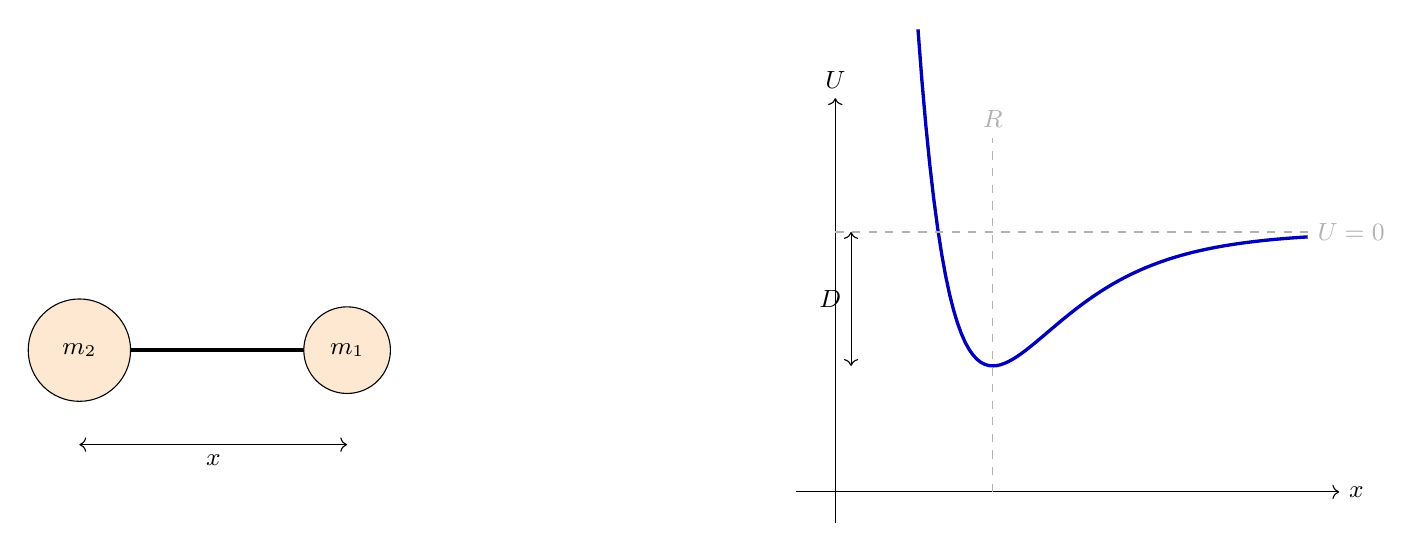
\begin{tikzpicture}[x=1cm,y=1cm,font=\small]

\begin{scope}[shift={(-4.2,0)}]
    \draw[draw=black,fill=orange!18] (-1.7,0) circle (.65) node {$m_2$};
    \draw[draw=black,fill=orange!18] (1.7,0) circle (.55) node {$m_1$};
    \draw[very thick] (-1.05,0)--(1.15,0);
    \draw[<->] (-1.7,-1.2)--(1.7,-1.2) node[midway,below] {$x$};
  \end{scope}
  \begin{scope}[shift={(3.7,-1.8)}]
    \draw[->] (-.5,0)--(6.4,0) node[right] {$x$};
    \draw[->] (0,-.4)--(0,5) node[above] {$U$};
    \draw[very thick,blue!70!black,domain=1.05:6,samples=100]
      plot (\x,{1.7*(exp(-2*(\x-2))-2*exp(-(\x-2)))+3.3});
    \draw[guide] (0,3.3)--(6,3.3) node[right] {$U=0$};
    \draw[guide] (2,0)--(2,4.5) node[above] {$R$};
    \draw[<->] (.2,1.6)--(.2,3.3) node[midway,left] {$D$};
  \end{scope}

\end{tikzpicture}

% 10 solution-05
\begin{tikzpicture}[x=1cm,y=1cm,font=\small]

\draw[axis](-2,0)--(5,0)node[right]{$\alpha q$};\draw[axis](0,-.2)--(0,3)node[above]{$(U+D)/D$};
\draw[orbit,domain=-.8:3.8,samples=120]plot(\x,{(1-exp(-\x))^2});
\draw[red!70!black,dashed,domain=-.8:1.1,samples=50]plot(\x,{(\x)^2});
\draw[guide](-.405465,.25)--(.693147,.25);\fill(-.405465,.25)circle(2pt);\fill(.693147,.25)circle(2pt);
\node[below]at(-.405465,-.1){$q_L$};\node[below]at(.693147,-.1){$q_R$};
\node[align=left,anchor=west]at(5.3,1.6){蓝：Morse；红：谐振近似\\示例 $\varepsilon/D=1/4$\\$q_L=-\ln(1+s)/\alpha$\\$q_R=-\ln(1-s)/\alpha$\\有限振幅不关于零对称};

\end{tikzpicture}

% 11 question-06
\begin{tikzpicture}[x=1cm,y=1cm,font=\small]
\fill[blue!6](-3,-2.8)rectangle(3,0);\draw[thick](-3,0)--(3,0);\draw[guide](0,-2.7)--(0,2.7);\draw[velocity](-2.1,2.1)--(0,0)node[pos=.25,left]{$\bm k_1$};\draw[velocity](0,0)--(2.1,2.1)node[right]{$\bm k_2$};\draw[velocity](0,0)--(1.27279,-2.38118)node[right]{$\bm k_3$};\draw[force](-1.10000,1.10000)--(-0.50000,1.70000)node[above]{$E_1$};\draw[force](1.10000,1.10000)--(0.50000,1.70000)node[above]{$E_2$};\draw[force](0.60000,-1.12250)--(1.21734,-0.79251)node[above]{$E_3$};\node[above left]at(-2.3,.15){$n_1$};\node[below left]at(-2.3,-.15){$n_2$};\node at(0,-3.1){$i=45^\circ,\gamma=28.13^\circ$ 示意};
\end{tikzpicture}

% 12 solution-06
\begin{tikzpicture}[x=1cm,y=1cm,font=\small]
\begin{scope}[shift={(-3.5,0)},scale=.8]\fill[blue!6](-3,-2.8)rectangle(3,0);\draw[thick](-3,0)--(3,0);\draw[guide](0,-2.7)--(0,2.7);\draw[velocity](-2.1,2.1)--(0,0)node[pos=.25,left]{$\bm k_1$};\draw[velocity](0,0)--(2.1,2.1)node[right]{$\bm k_2$};\draw[velocity](0,0)--(1.27279,-2.38118)node[right]{$\bm k_3$};\draw[force](-1.10000,1.10000)--(-0.50000,1.70000)node[above]{$E_1$};\draw[force](1.10000,1.10000)--(0.50000,1.70000)node[above]{$E_2$};\draw[force](0.60000,-1.12250)--(1.21734,-0.79251)node[above]{$E_3$};\node[above left]at(-2.3,.15){$n_1$};\node[below left]at(-2.3,-.15){$n_2$};\node at(0,-3.1){$i=45^\circ,\gamma=28.13^\circ$ 示意};\end{scope}\begin{scope}[shift={(.2,-1.3)}]\draw[axis](0,0)--(5.5,0)node[right]{$i$};\draw[axis](0,-2.3)--(0,1)node[above]{$r_p$};\draw[orbit]plot coordinates{(0.00000,0.40000) (0.02507,0.39998) (0.05014,0.39993) (0.07521,0.39985) (0.10028,0.39974) (0.12535,0.39959) (0.15042,0.39940) (0.17549,0.39919) (0.20056,0.39894) (0.22563,0.39866) (0.25070,0.39834) (0.27577,0.39799) (0.30084,0.39761) (0.32591,0.39719) (0.35098,0.39674) (0.37605,0.39626) (0.40112,0.39574) (0.42619,0.39518) (0.45126,0.39460) (0.47633,0.39397) (0.50140,0.39331) (0.52647,0.39262) (0.55154,0.39189) (0.57661,0.39113) (0.60168,0.39033) (0.62674,0.38949) (0.65181,0.38862) (0.67688,0.38771) (0.70195,0.38676) (0.72702,0.38578) (0.75209,0.38476) (0.77716,0.38370) (0.80223,0.38260) (0.82730,0.38147) (0.85237,0.38029) (0.87744,0.37908) (0.90251,0.37783) (0.92758,0.37653) (0.95265,0.37520) (0.97772,0.37382) (1.00279,0.37241) (1.02786,0.37095) (1.05293,0.36945) (1.07800,0.36790) (1.10307,0.36631) (1.12814,0.36468) (1.15321,0.36301) (1.17828,0.36128) (1.20335,0.35952) (1.22842,0.35770) (1.25349,0.35584) (1.27856,0.35394) (1.30363,0.35198) (1.32870,0.34998) (1.35377,0.34792) (1.37884,0.34582) (1.40391,0.34366) (1.42898,0.34146) (1.45405,0.33920) (1.47912,0.33688) (1.50419,0.33452) (1.52926,0.33209) (1.55433,0.32961) (1.57940,0.32708) (1.60447,0.32449) (1.62954,0.32184) (1.65461,0.31913) (1.67968,0.31635) (1.70475,0.31352) (1.72982,0.31063) (1.75489,0.30767) (1.77996,0.30464) (1.80503,0.30155) (1.83009,0.29839) (1.85516,0.29517) (1.88023,0.29187) (1.90530,0.28851) (1.93037,0.28507) (1.95544,0.28156) (1.98051,0.27797) (2.00558,0.27430) (2.03065,0.27056) (2.05572,0.26674) (2.08079,0.26284) (2.10586,0.25886) (2.13093,0.25479) (2.15600,0.25064) (2.18107,0.24640) (2.20614,0.24207) (2.23121,0.23765) (2.25628,0.23314) (2.28135,0.22853) (2.30642,0.22383) (2.33149,0.21902) (2.35656,0.21412) (2.38163,0.20911) (2.40670,0.20400) (2.43177,0.19879) (2.45684,0.19346) (2.48191,0.18802) (2.50698,0.18247) (2.53205,0.17680) (2.55712,0.17101) (2.58219,0.16510) (2.60726,0.15907) (2.63233,0.15291) (2.65740,0.14662) (2.68247,0.14019) (2.70754,0.13363) (2.73261,0.12693) (2.75768,0.12009) (2.78275,0.11310) (2.80782,0.10597) (2.83289,0.09868) (2.85796,0.09124) (2.88303,0.08363) (2.90810,0.07587) (2.93317,0.06793) (2.95824,0.05983) (2.98331,0.05155) (3.00838,0.04309) (3.03345,0.03445) (3.05851,0.02562) (3.08358,0.01660) (3.10865,0.00738) (3.13372,-0.00204) (3.15879,-0.01167) (3.18386,-0.02152) (3.20893,-0.03157) (3.23400,-0.04186) (3.25907,-0.05237) (3.28414,-0.06311) (3.30921,-0.07410) (3.33428,-0.08533) (3.35935,-0.09681) (3.38442,-0.10856) (3.40949,-0.12057) (3.43456,-0.13285) (3.45963,-0.14541) (3.48470,-0.15826) (3.50977,-0.17141) (3.53484,-0.18485) (3.55991,-0.19861) (3.58498,-0.21269) (3.61005,-0.22710) (3.63512,-0.24184) (3.66019,-0.25693) (3.68526,-0.27237) (3.71033,-0.28818) (3.73540,-0.30436) (3.76047,-0.32093) (3.78554,-0.33790) (3.81061,-0.35527) (3.83568,-0.37306) (3.86075,-0.39128) (3.88582,-0.40995) (3.91089,-0.42907) (3.93596,-0.44866) (3.96103,-0.46873) (3.98610,-0.48930) (4.01117,-0.51037) (4.03624,-0.53198) (4.06131,-0.55413) (4.08638,-0.57683) (4.11145,-0.60011) (4.13652,-0.62398) (4.16159,-0.64846) (4.18666,-0.67357) (4.21173,-0.69933) (4.23680,-0.72575) (4.26186,-0.75287) (4.28693,-0.78069) (4.31200,-0.80925) (4.33707,-0.83857) (4.36214,-0.86866) (4.38721,-0.89956) (4.41228,-0.93130) (4.43735,-0.96389) (4.46242,-0.99737) (4.48749,-1.03177) (4.51256,-1.06712) (4.53763,-1.10345) (4.56270,-1.14080) (4.58777,-1.17920) (4.61284,-1.21868) (4.63791,-1.25929) (4.66298,-1.30106) (4.68805,-1.34404) (4.71312,-1.38827) (4.73819,-1.43379) (4.76326,-1.48066) (4.78833,-1.52892) (4.81340,-1.57863) (4.83847,-1.62984) (4.86354,-1.68261) (4.88861,-1.73701) (4.91368,-1.79308) (4.93875,-1.85091) (4.96382,-1.91055) (4.98889,-1.97210)};\draw[red!70!black,thick,dashed]plot coordinates{(0.00000,0.08000) (0.02507,0.07999) (0.05014,0.07997) (0.07521,0.07994) (0.10028,0.07989) (0.12535,0.07983) (0.15042,0.07976) (0.17549,0.07968) (0.20056,0.07958) (0.22563,0.07946) (0.25070,0.07934) (0.27577,0.07920) (0.30084,0.07905) (0.32591,0.07888) (0.35098,0.07870) (0.37605,0.07851) (0.40112,0.07830) (0.42619,0.07809) (0.45126,0.07785) (0.47633,0.07761) (0.50140,0.07735) (0.52647,0.07708) (0.55154,0.07679) (0.57661,0.07649) (0.60168,0.07618) (0.62674,0.07585) (0.65181,0.07551) (0.67688,0.07516) (0.70195,0.07479) (0.72702,0.07441) (0.75209,0.07402) (0.77716,0.07361) (0.80223,0.07319) (0.82730,0.07276) (0.85237,0.07231) (0.87744,0.07185) (0.90251,0.07138) (0.92758,0.07089) (0.95265,0.07039) (0.97772,0.06987) (1.00279,0.06934) (1.02786,0.06880) (1.05293,0.06825) (1.07800,0.06768) (1.10307,0.06709) (1.12814,0.06650) (1.15321,0.06589) (1.17828,0.06526) (1.20335,0.06463) (1.22842,0.06398) (1.25349,0.06331) (1.27856,0.06264) (1.30363,0.06195) (1.32870,0.06124) (1.35377,0.06052) (1.37884,0.05979) (1.40391,0.05905) (1.42898,0.05830) (1.45405,0.05753) (1.47912,0.05674) (1.50419,0.05595) (1.52926,0.05514) (1.55433,0.05432) (1.57940,0.05349) (1.60447,0.05265) (1.62954,0.05179) (1.65461,0.05092) (1.67968,0.05004) (1.70475,0.04915) (1.72982,0.04824) (1.75489,0.04733) (1.77996,0.04640) (1.80503,0.04547) (1.83009,0.04452) (1.85516,0.04356) (1.88023,0.04259) (1.90530,0.04162) (1.93037,0.04063) (1.95544,0.03964) (1.98051,0.03863) (2.00558,0.03762) (2.03065,0.03660) (2.05572,0.03558) (2.08079,0.03454) (2.10586,0.03350) (2.13093,0.03246) (2.15600,0.03141) (2.18107,0.03036) (2.20614,0.02930) (2.23121,0.02824) (2.25628,0.02718) (2.28135,0.02611) (2.30642,0.02505) (2.33149,0.02399) (2.35656,0.02292) (2.38163,0.02186) (2.40670,0.02081) (2.43177,0.01976) (2.45684,0.01871) (2.48191,0.01768) (2.50698,0.01665) (2.53205,0.01563) (2.55712,0.01462) (2.58219,0.01363) (2.60726,0.01265) (2.63233,0.01169) (2.65740,0.01075) (2.68247,0.00983) (2.70754,0.00893) (2.73261,0.00806) (2.75768,0.00721) (2.78275,0.00640) (2.80782,0.00561) (2.83289,0.00487) (2.85796,0.00416) (2.88303,0.00350) (2.90810,0.00288) (2.93317,0.00231) (2.95824,0.00179) (2.98331,0.00133) (3.00838,0.00093) (3.03345,0.00059) (3.05851,0.00033) (3.08358,0.00014) (3.10865,0.00003) (3.13372,0.00000) (3.15879,0.00007) (3.18386,0.00023) (3.20893,0.00050) (3.23400,0.00088) (3.25907,0.00137) (3.28414,0.00199) (3.30921,0.00275) (3.33428,0.00364) (3.35935,0.00469) (3.38442,0.00589) (3.40949,0.00727) (3.43456,0.00882) (3.45963,0.01057) (3.48470,0.01252) (3.50977,0.01469) (3.53484,0.01709) (3.55991,0.01972) (3.58498,0.02262) (3.61005,0.02579) (3.63512,0.02924) (3.66019,0.03301) (3.68526,0.03709) (3.71033,0.04152) (3.73540,0.04632) (3.76047,0.05150) (3.78554,0.05709) (3.81061,0.06311) (3.83568,0.06959) (3.86075,0.07655) (3.88582,0.08403) (3.91089,0.09205) (3.93596,0.10065) (3.96103,0.10985) (3.98610,0.11971) (4.01117,0.13024) (4.03624,0.14150) (4.06131,0.15353) (4.08638,0.16637) (4.11145,0.18007) (4.13652,0.19468) (4.16159,0.21025) (4.18666,0.22685) (4.21173,0.24453) (4.23680,0.26336) (4.26186,0.28340) (4.28693,0.30474) (4.31200,0.32744) (4.33707,0.35160) (4.36214,0.37729) (4.38721,0.40461) (4.41228,0.43366) (4.43735,0.46454) (4.46242,0.49738) (4.48749,0.53228) (4.51256,0.56938) (4.53763,0.60881) (4.56270,0.65071) (4.58777,0.69525) (4.61284,0.74259) (4.63791,0.79290) (4.66298,0.84638) (4.68805,0.90322) (4.71312,0.96364) (4.73819,1.02788) (4.76326,1.09618) (4.78833,1.16880) (4.81340,1.24604) (4.83847,1.32820) (4.86354,1.41560) (4.88861,1.50859) (4.91368,1.60757) (4.93875,1.71293) (4.96382,1.82511) (4.98889,1.94458)};\node[blue]at(1,1.3){$r_p$};\node[red!70!black]at(3,1.3){$\mathcal R=r_p^2$};\draw[guide](3.1283,-2.1)--(3.1283,.6);\node[above]at(3.1283,.6){$i_B=56.31^\circ$};\node[below]at(5,0){$90^\circ$};\node[align=center]at(2.7,-2.9){按各光束正偏振基定义\\掠入射 $r_p\to-1$，法向电场反相};\end{scope}
\end{tikzpicture}

% 13 question-07
\begin{tikzpicture}[x=1cm,y=1cm,font=\small]

\draw[thick](0,3)--(1,3);\node[left]at(0,3){$a$};
\draw[thick](1,3)--(1.65,3) (2.35,3)--(3,3);\draw[body](1.65,2.82)rectangle(2.35,3.18);\node at(2.0,3){$R_x$};\draw[thick](3,3)--(3.8,3);\fill(3.5,3)circle(2pt)node[above]{$b$};
\draw[thick](4.15,3)circle(.35)node{$A$};\draw[thick](4.5,3)--(5,3);\fill(4.8,3)circle(2pt)node[above]{$c$};
\draw[thick](5,3)--(5.65,3) (6.35,3)--(7,3);\draw[body](5.65,2.82)rectangle(6.35,3.18);\node at(6.0,3){$R_0$};\draw[thick](7,3)--(7.5,3)--(7.5,1.6);\fill(7.5,3)circle(2pt)node[right]{$d$};
\draw[thick](0,3)--(0,0)--(2.7,0);\draw[thick](2.7,-.4)--(2.7,.4) (3,-.25)--(3,.25);\draw[thick](3,0)--(5.2,0);\node[below]at(2.9,-.5){$\varepsilon,r$};
\draw[thick](7.5,1.6)--(6.7,1.6);\fill(6.7,1.6)circle(2pt)node[above]{$K_1$公共端 $d$};
\draw[thick](6.7,1.6)--(5.8,2);\draw[terminal](5.5,2.2)circle(.06)node[above]{2};\draw[thick](5.5,2.2)--(3.5,2.2)--(3.5,3);
\draw[terminal](5.5,1.2)circle(.06)node[below]{1};\draw[thick](5.5,1.2)--(.6,1.2)--(.6,3);
\fill(5.2,0)circle(2pt)node[below]{$K_2$公共端 $-$};\draw[thick](5.2,0)--(6.1,.45);
\draw[terminal](6.4,.65)circle(.06)node[above]{3};\draw[thick](6.4,.65)--(8.2,.65)--(8.2,3)--(7.5,3);
\draw[terminal](6.4,-.65)circle(.06)node[below]{4};\draw[thick](6.4,-.65)--(4.8,-.65)--(4.8,3);
\node[align=center]at(3.8,-1.55){$K_1$可断开“空”；闭合状态由触点表规定\\$K_1=1,K_2=3$ 将短接电源，禁止};

\fill(.6,3)circle(2pt);\node at(4.1,-2.1){有圆点为连接；相交无圆点的导线不连接};
\end{tikzpicture}

% 14 solution-07
\begin{tikzpicture}[x=1cm,y=1cm,font=\small]
\begin{scope}[shift={(0.0,0.0)}]\node[anchor=west]at(0,1.65){A：空/3，$I_1$};\fill(0,0)circle(2pt);\node[left]at(0,0){$+$};\fill(5.5,0)circle(2pt);\node[right]at(5.5,0){$-$};\draw[thick](0,0)--(0.55,0) (1.25,0)--(1.8,0);\draw[body](0.55,-0.18)rectangle(1.25,0.18);\node at(0.9,0){$R_x$};\draw[thick](1.8,0)--(2.35,0);\draw[thick](2.8,0)circle(.45)node{$A$};\draw[thick](3.25,0)--(3.7,0);\draw[thick](3.7,0)--(4.25,0) (4.949999999999999,0)--(5.5,0);\draw[body](4.25,-0.18)rectangle(4.949999999999999,0.18);\node at(4.6,0){$R_0$};\end{scope}\begin{scope}[shift={(6.4,0.0)}]\node[anchor=west]at(0,1.65){B：空/4，$I_2$};\fill(0,0)circle(2pt);\node[left]at(0,0){$+$};\fill(5.5,0)circle(2pt);\node[right]at(5.5,0){$-$};\draw[thick](0,0)--(0.55,0) (1.25,0)--(1.8,0);\draw[body](0.55,-0.18)rectangle(1.25,0.18);\node at(0.9,0){$R_x$};\draw[thick](1.8,0)--(2.35,0);\draw[thick](2.8,0)circle(.45)node{$A$};\draw[thick](3.25,0)--(3.7,0);\draw[thick](3.7,0)--(5.5,0);\end{scope}\begin{scope}[shift={(0.0,-3.4)}]\node[anchor=west]at(0,1.65){C：2/4，$I_3$};\fill(0,0)circle(2pt);\node[left]at(0,0){$+$};\fill(5.5,0)circle(2pt);\node[right]at(5.5,0){$-$};\draw[thick](0,0)--(0.65,0) (1.35,0)--(2.0,0);\draw[body](0.65,-0.18)rectangle(1.35,0.18);\node at(1.0,0){$R_x$};\draw[thick](2.0,0)--(2.0,.7)--(2.35,.7);\draw[thick](2.8,.7)circle(.45)node{$A$};\draw[thick](3.25,.7)--(4.8,.7)--(4.8,-.7);\draw[thick](2.0,0)--(2.0,-.7);\draw[thick](2.0,-0.7)--(3.05,-0.7) (3.75,-0.7)--(4.8,-0.7);\draw[body](3.05,-0.8799999999999999)rectangle(3.75,-0.52);\node at(3.4,-0.7){$R_0$};\draw[thick](4.8,0)--(5.5,0);\fill(2.0,0)circle(2pt);\fill(4.8,0)circle(2pt);\end{scope}\begin{scope}[shift={(6.4,-3.4)}]\node[anchor=west]at(0,1.65){D：1/4，$I_4$};\fill(0,0)circle(2pt);\node[left]at(0,0){$+$};\fill(5.5,0)circle(2pt);\node[right]at(5.5,0){$-$};\draw[thick](0,0)--(0.65,0);\draw[thick](0.65,0)--(0.65,.7);\draw[thick](0.65,0.7)--(0.975,0.7) (1.6749999999999998,0.7)--(2.0,0.7);\draw[body](0.975,0.52)rectangle(1.6749999999999998,0.8799999999999999);\node at(1.325,0.7){$R_x$};\draw[thick](2,.7)--(2.35,.7);\draw[thick](2.8,.7)circle(.45)node{$A$};\draw[thick](3.25,.7)--(4.8,.7)--(4.8,-.7);\draw[thick](0.65,0)--(0.65,-.7);\draw[thick](0.65,-0.7)--(2.375,-0.7) (3.075,-0.7)--(4.8,-0.7);\draw[body](2.375,-0.8799999999999999)rectangle(3.075,-0.52);\node at(2.725,-0.7){$R_0$};\draw[thick](4.8,0)--(5.5,0);\fill(0.65,0)circle(2pt);\fill(4.8,0)circle(2pt);\end{scope}\node[align=center]at(5.7,-5.1){四图为负载等效网络，电源的 $\varepsilon,r$ 位于端口外；$A$ 含内阻 $r_g$\\A、B中电流不分流；C、D中 $I_3,I_4$ 为表头支路电流};
\end{tikzpicture}

% 15 question-08
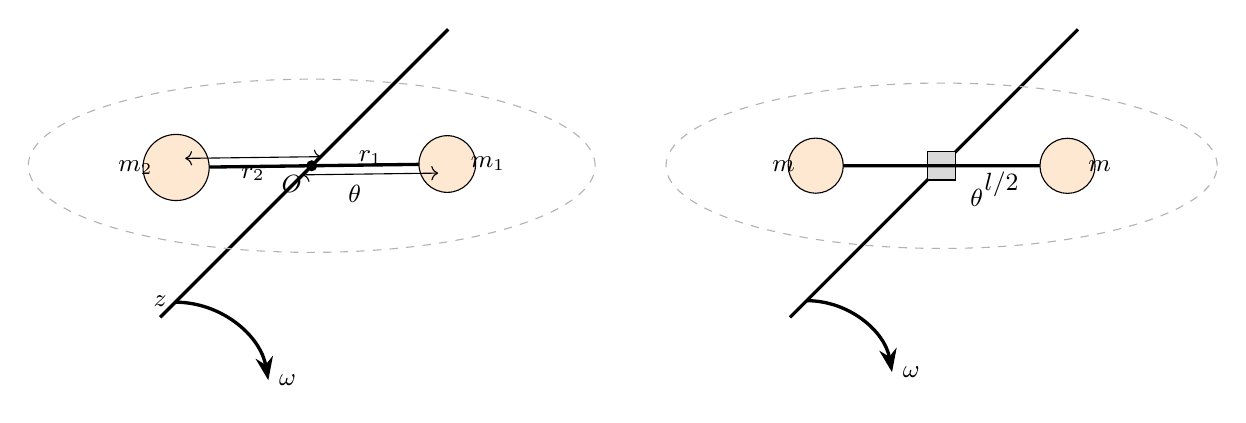
\begin{tikzpicture}[x=1cm,y=1cm,font=\small]

\draw[very thick] (0,0,-4.5)--(0,0,5) node[above] {$z$};
  \draw[guide] (0,0,0) ellipse (3.6 and 1.1);
  \draw[very thick] (-2.8,-1.1,-2.8)--(0,0,0)--(2.8,1.1,2.8);
  \draw[draw=black,fill=orange!18] (-2.8,-1.1,-2.8) circle (.42) node[left=5pt] {$m_2$};
  \draw[draw=black,fill=orange!18] (2.8,1.1,2.8) circle (.36) node[right=5pt] {$m_1$};
  \fill (0,0,0) circle (2pt) node[below left] {$O$};
  \draw[<->] (0,0,.3)--(2.8,1.1,3.1) node[midway,above] {$r_1$};
  \draw[<->] (-2.8,-1.1,-3.1)--(0,0,-.3) node[midway,below] {$r_2$};
  \draw[vec] (0,0,4.5) arc (90:10:1.2) node[right] {$\omega$};
  \node at (1.2,.3,1.7) {$\theta$};
  \begin{scope}[shift={(8,0,0)}]
    \draw[very thick] (0,0,-4.5)--(0,0,5);
    \draw[guide] (0,0,0) ellipse (3.5 and 1.05);
    \draw[fill=gray!30] (-.45,-.45,-.7) rectangle (.45,.45,.7);
    \draw[very thick] (-2.6,-1,-2.6)--(2.6,1,2.6);
    \draw[draw=black,fill=orange!18] (-2.6,-1,-2.6) circle (.35)
      node[left=4pt] {$m$};
    \draw[draw=black,fill=orange!18] (2.6,1,2.6) circle (.35)
      node[right=4pt] {$m$};
    \node at (1.55,.55,2.05) {$l/2$};
    \node at (1.1,.25,1.7) {$\theta$};
    \draw[vec] (0,0,4.45) arc (90:10:1.1) node[right] {$\omega$};
  \end{scope}

\end{tikzpicture}

% 16 solution-08
\begin{tikzpicture}[x=1cm,y=1cm,font=\small]

\draw[axis](0,-.3)--(0,3.8)node[above]{$\hat{\bm z}$};\draw[axis](-.3,0)--(3.7,0)node[right]{$\hat{\bm e}_r$};
\draw[very thick](0,0)--(2.6,2.6)node[right]{$\bm n$};\draw[guide](0,0)circle(.7);\node at(.4,.9){$\theta$};
\draw[velocity](0,0)--(0,2)node[left]{$L_z$};\draw[force](0,0)--(-2,2)node[left]{$\bm L$};\draw[guide](-2,2)--(0,2);
\node[draw,circle,inner sep=2pt]at(2.8,.5){$\otimes$};\node[right]at(3.3,.5){$\bm\tau\parallel-\hat{\bm e}_\phi$};
\node[align=left,anchor=west]at(4.4,2.6){$K=ml^2/2$\\$\bm L=K\omega(\hat{\bm z}-\cos\theta\,\bm n)$\\$L_z=K\omega\sin^2\theta=\mathrm{const}$\\$\bm\tau=-K\omega^2\sin\theta\cos\theta\,\hat{\bm e}_\phi$\\示意 $0<\theta<\pi/2,\omega>0$\\轴力矩无竖直分量，且不做功};

\end{tikzpicture}

\end{document}
